\section{Diagramas Arquiteturais}\label{sec:diagramas}
As Figuras~\ref{fig:contexto}--\ref{fig:demo} oferecem vistas complementares.
A Figura~\ref{fig:sequencia} detalha a leitura local e a gravação do favorito;
a sincronização remota é um fluxo complementar, não uma chamada direta do
ViewModel à rede. Os fontes Mermaid e as exportações vetoriais acompanham a
entrega para revisão das relações.

\begin{figure*}[t]
\centering
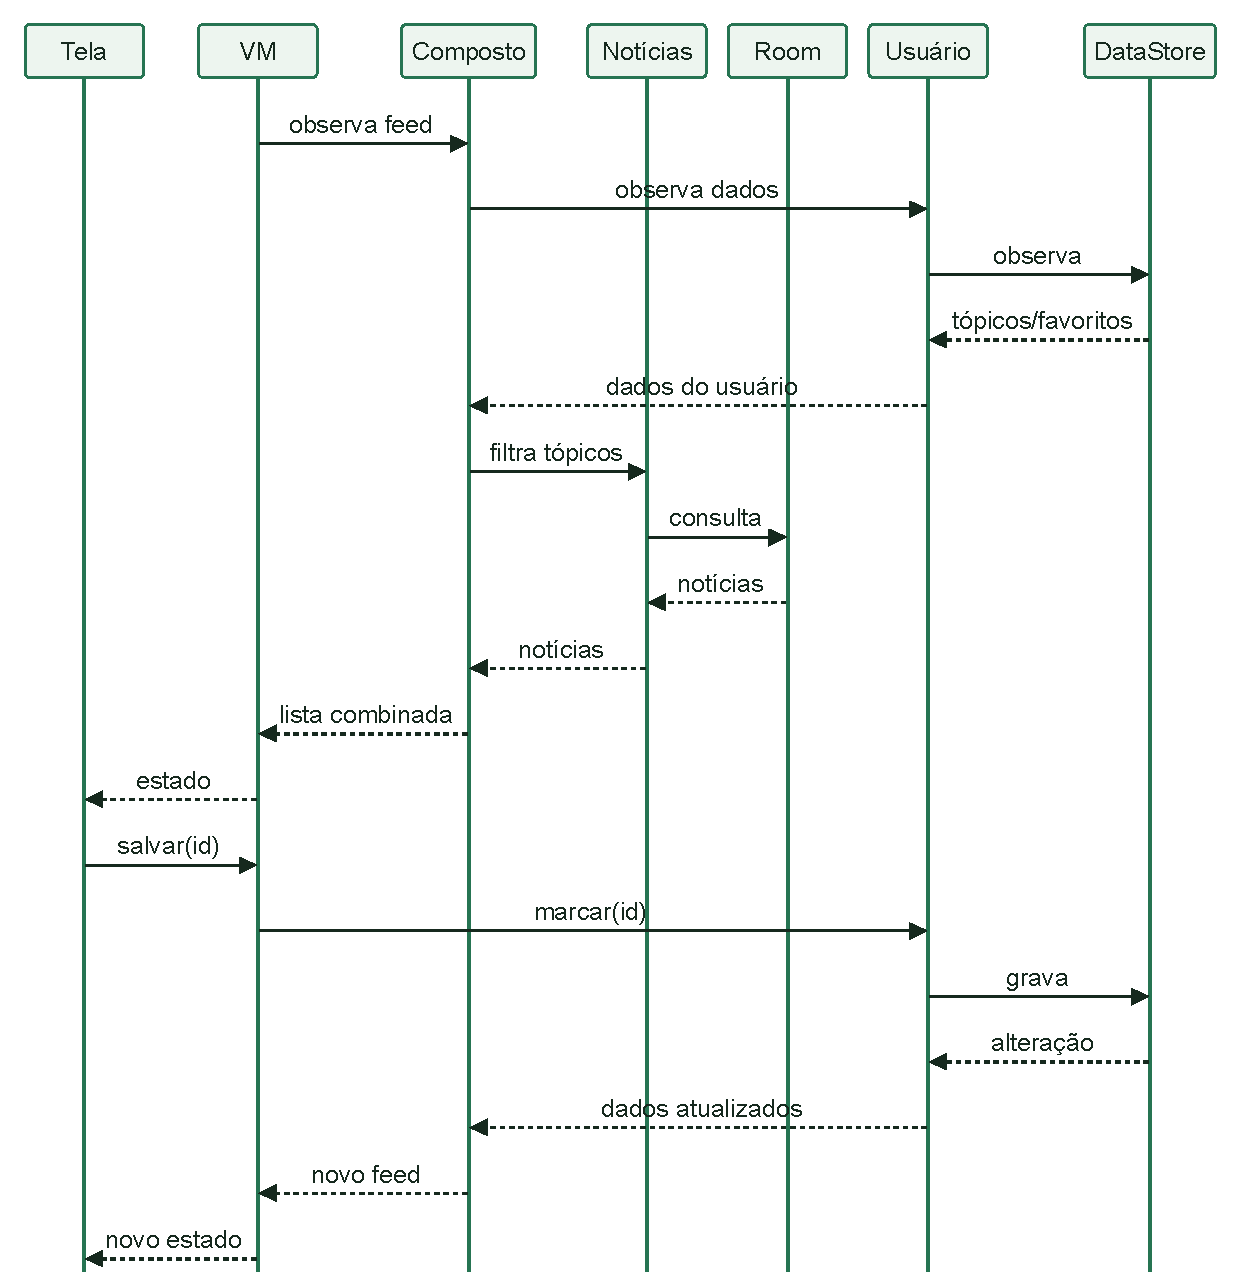
\includegraphics[width=.90\textwidth]{imagens/04-sequencia.pdf}
\caption{Sequência atual do recorte For You. ``Composto'' representa
CompositeUserNewsResourceRepository; ``Notícias'' e ``Usuário'' representam
seus repositórios. O desenho omite onboarding, analytics e detalhes internos.}
\Description{O ViewModel observa o feed combinado de notícias Room e preferências DataStore. A ação de salvar passa pelo repositório de usuário; a nova emissão recompõe o estado.}
\label{fig:sequencia}
\end{figure*}
